% ------------------------------------------------------------------------------
% ------------------------------------------------------------------------------
% Relatório de Trabalho 1 de Algoritmos Numéricos 2
% Autor: André Barreto Silveira
% ------------------------------------------------------------------------------
% ------------------------------------------------------------------------------

\documentclass[
	11pt,				% tamanho da fonte
	oneside,			% para impressão apenas no verso. Oposto a twoside
	a4paper,			% tamanho do papel. 
	english,			% idioma adicional para hifenização
	brazil,				% o último idioma é o principal do documento
	]{article}


% ---
% PACOTES
% ---
\usepackage{lmodern}
\usepackage[T1]{fontenc}
\usepackage[utf8]{inputenc}
\usepackage{indentfirst}
\usepackage{nomencl}
\usepackage{color}
\usepackage{graphicx}
\usepackage{microtype}
\usepackage{makeidx}
\usepackage{multirow,tabularx}
\usepackage{multicol}
\usepackage{listings}
\usepackage{color}
\usepackage{hyperref}
\usepackage{cite}
\usepackage{url}
\usepackage[brazilian]{babel}
\usepackage[brazilian,hyperpageref]{backref}
\usepackage[fleqn]{amsmath}
\usepackage{mathtools,amssymb}
\usepackage{pgfplots}

\usepackage{lipsum}
% ---

% ---
% Configurações do pacote listings
% ---
\definecolor{mygreen}{rgb}{0,0.6,0}
\definecolor{mygray}{rgb}{0.571428571,0.571428571,0.571428571}
\definecolor{mymauve}{rgb}{0.5714285718,0,0.82}
\definecolor{codegreen}{rgb}{0,0.6,0}
\definecolor{codegray}{rgb}{0.571428571,0.571428571,0.571428571}
\definecolor{codepurple}{rgb}{0.5714285718,0,0.82}
\definecolor{backcolour}{rgb}{0.95,0.95,0.92}
\lstset{
	backgroundcolor=\color{white},
	basicstyle=\footnotesize,
	breakatwhitespace=false,
	breaklines=true,
	captionpos=b,
	commentstyle=\color{mygreen},
	deletekeywords={...},
	escapeinside={\%*}{*)},
	extendedchars=true,
	keepspaces=true,
	keywordstyle=\color{blue},
	language=C,
	otherkeywords={*,...},
	numbers=left,
	numbersep=5pt,
	numberstyle=\tiny\color{mygray},
	rulecolor=\color{black},
	showspaces=false,
	showstringspaces=false,
	showtabs=false,
	stepnumber=1,
	stringstyle=\color{mymauve},
	tabsize=2,
	title=\lstname
}
% ---
	
% ---
% Informações de dados para CAPA
% ---
\title{\textbf{Solução de Problemas de Valor no Contorno Bidimensionais}}
\author{
André Barreto e Igor Ventorim\\\\
\normalsize Universidade Federal do Espírito Santo\\
}
\date{2015}
% ---

% ---
% Configurações de aparência do PDF final
% ---
\definecolor{blue}{RGB}{41,5,195}

% informações do PDF
\makeatletter
\hypersetup{
	pdftitle={\@title}, 
	pdfauthor={\@author},
	pdfsubject={Escalonamento de Jobs},
	pdfcreator={LaTeX with abnTeX2},
	pdfkeywords={abnt}{latex}{abntex}{abntex2}{atigo científico}, 
	colorlinks=true,
	linkcolor=blue,
	citecolor=blue,
	filecolor=magenta,
	urlcolor=blue,
	bookmarksdepth=4
}
\makeatother
% --- 

% ---
% Compila o indice
% ---
\makeindex
% ---

% --- 
% Espaçamentos entre linhas e parágrafos 
% --- 
\setlength{\parindent}{1cm}
\setlength{\parskip}{0.2cm}
% ---

% ----
% Início do documento
% ----
\begin{document}
% ---

% Seleciona o idioma do documento
\selectlanguage{brazil}

% Retira espaço extra obsoleto entre as frases.
\frenchspacing

\graphicspath{ {Imagens/} }

% ------------------------------------------------------------------------------
% Página de Título
% ------------------------------------------------------------------------------
\begin{titlepage}
	\centering
	{\scshape \large Universidade Federal do Espírito Santo\par}
	{\large Departamento de Informática\par}
	\vspace{1cm}
	{\large André Barreto Silveira\par}
	
	\vfill
	
	{\LARGE \bfseries Método das Diferenças Finitas Aplicado a
Problemas Bidimensionais\par}
	\vspace{1cm}
	{\large Trabalho 1 de Algoritmos Numéricos 2\par}

	\vfill

	{\large Vitória\par}
	{\large 2016\par}
\end{titlepage}
\addtocounter{page}{1}

% ------------------------------------------------------------------------------
% Introdução
% ------------------------------------------------------------------------------
\section{Introdução}
O estudo da equação de transporte, também denominada equação da 
advecção-difusão-reação, continua sendo um ativo campo de pesquisa, uma vez que 
essa equação é de fundamental importância nos problemas relacionados a 
aerodinâmica,  meteorologia, oceanografia, hidrologia, engenharia química e
de reservatórios. A equação de transporte tem características bastante 
peculiares que fazem com que sua  resolução por meios numéricos seja 
dificultada em situações onde o problema é fortemente convectivo. Por isso, 
diversos métodos têm sido desenvolvidos e aplicados, com a intenção de superar 
as dificuldades numéricas impostas por esta equação.

A equação de transporte bidimensional pode ser definida por:

\begin{equation} \label{eq:transporte}
- k \left(\frac{\partial^2 u}{\partial x^2} + \frac{\partial^2 u}{\partial 
y^2}\right) +
\beta_x(x,y)\frac{\partial u}{\partial x} +
\beta_y(x,y)\frac{\partial u}{\partial y} +
\gamma(x,y)u = f(x,y) \text{ em } \Omega
\end{equation}

Este trabalho tem como objetivo verificar como as formas de armazenamento das 
estruturas resultantes pela discretização da equação \eqref{eq:transporte} por 
diferenças finitas pode impactar no tempo de processamento.

Para isto, será implementado em linguagem C um programa capaz de aplicar a 
discretização da equação de transporte e resolver o sistema resultante 
discreto. Quanto ao método de resolução, será aplicado o algoritmo SOR
(\textit{Sucessive Over Relaxation}) de duas formas: resolvendo o sistema 
penta-diagonal armazenado de forma esparsa, utilizando  cinto vetores; e 
completamente livre de matriz.

Nas próximas seções estão descritos em detalhes o desenvolvimento, testes e 
conceitos do trabalho, sendo que o próximo tópico faz um resumo do método das 
Diferenças Finitas, descrevendo as técnicas e ordem de aproximação usadas.

% ------------------------------------------------------------------------------
% Método das Diferenças Finitas
% ------------------------------------------------------------------------------
\section{Método das Diferenças Finitas}
Método das Diferenças Finitas é um método numérico para resolver equações 
diferenciais através de aproximações de derivadas por diferenças finitas. Estas 
aproximações são obtidas pela série de Taylor:
\begin{align*}
f(x+h) &= f(x)+f'(x)h + \frac{f''(x)h^2}{2} + \frac{f'''(x)h^3}{6} + o(h^4) \\ 
f(x-h) &= f(x) - f'(x)h + \frac{f''(x)h^2}{2} - \frac{f'''(x)h^3}{6} + 
o(h^4)
\end{align*}

Portanto, a primeira e segunda derivadas podem ser escritas das
seguintes formas:
\begin{align*}
f'(x) &= \frac{f(x+h)-f(x)}{h}+o(h) \text{ , diferença atrasada
(1ª ordem) }  \\
f'(x) &= \frac{f(x) - f(x-h)}{h} + o(h) \text{ , diferença adiantada
(1ª ordem) } \\
f'(x) &= \frac{f(x+h) - f(x-h)}{2h} + o(h^2) \text{ , diferença central 
(2ª ordem) } \\
f''(x) &= \frac{f(x+h) -2f(x) + f(x-h)}{h^2} + o(h^2)
\end{align*}

O método das Diferenças Finitas em domínios retangulares consiste em 
\textbf{três} etapas principais:

\begin{itemize}
 \item \textbf{Discretização do domínio}, onde os pontos $(x,y)$ são traduzidos 
em um domínio linear, de forma que $I = (j-1)n + i$ e $ 1 \le I \ge n*m$, onde 
$i$ e $j$ são representam um ponto bidimensional e $I$ uma posição 
representativa deste ponto.
 \item \textbf{Aproximar a Equação \eqref{eq:transporte} por diferenças 
finitas}, que consiste em reescrever a equação utilizando as aproximações por 
diferenças finitas, gerando um sistema linear.
 \item \textbf{Aplicar condições de contorno} que são definidas pelo problema 
proposto e que impactam diretamente na solução do problema.
\end{itemize}

Após a aplicação das etapas acima, teremos como resultado um sistema 
penta-diagonal da seguinte forma:
\begin{equation} \label{eq:discret}
e_Iu_{I-n} + c_Iu_{I-1} + a_Iu_I + b_Iu_{I+1} + d_Iu_{I+n} = f_I
\end{equation}

\noindent onde
\begin{align*}
e_I &= \left[\frac{-1}{h^2_y} - \frac{\beta_y}{2h_y}\right]  \\
c_I &= \left[\frac{-1}{h^2_x} - \frac{\beta_x}{2h_x}\right]  \\
a_I &= \left[\gamma_I + \frac{2}{h^2_x} + \frac{2}{h^2_y}\right]  \\
b_I &= \left[\frac{-1}{h^2_x} + \frac{\beta_x}{2h_x}\right]  \\
d_I &= \left[\frac{-1}{h^2_x} + \frac{\beta_y}{2h_y}\right]
\end{align*}

\noindent e a matriz de coeficientes é penta-diagonal, como ilustrado a seguir:

$
\begin{pmatrix}
	a_1     & c_1     &         & e_1     &         &         &         &        
 &         \\
	b_2     & a_2     & c_2     &         & e_2     &         &         &        
 &         \\
	        & \ddots  & \ddots  & \ddots  &         & \ddots  &         &        
 &         \\
	d_{n+1} &         & b_{n+1} & a_{n+1} & c_{n+1} &         & e_{n+1} &        
 &         \\
	        & \ddots  &         & \ddots  & \ddots  & \ddots  &         & \ddots 
 &         \\
	        &         & d_I     &         & b_I     & a_I     & c_I     &        
 & e_I     \\
	        &         &         & \ddots  &         & \ddots  & \ddots  & \ddots 
 &         \\
	        &         &         & d_{N-1} &         &         & b_{N-1} & 
a_{N-1} & c_{N-1} \\
	        &         &         &         & d_N     &         &         & b_N    
 & a_N     \\
\end{pmatrix}
$


% ------------------------------------------------------------------------------
% Implementação
% ------------------------------------------------------------------------------
\section{Implementação}
Nesta seção estão apresentados os códigos em C relevantes do sistema que mostra 
suas principais funcionalidades necessárias para a resolução do Método das 
Diferenças Finitas Bidimensional.

O sistema foi desenvolvido com base nas três principais etapas do método das 
diferenças finitas: discretizar o domínio, realizar a aproximação por 
diferenças finitas e aplicar condições de contorno. Em todos os experimentos 
estas etapas são necessárias, porém, devido às diferenças algorítmicas entre os 
experimentos, o programa seria muito complexo se fosse feito de forma genérica. 
Por conta disto, e almejando um programa eficiente para a solução dos problemas, 
o código foi escrito de forma condicional, onde dependendo do experimento 
indicado para resolver, partes diferentes do programa serão utilizadas. Isto 
implica em um código de baixa manutenibilidade, devido à grande repetição de 
códigos, mas ganha em eficiência, como desejado.

\subsection{Estruturas}
Estão ilustradas nesta seção as estruturas de dados utilizadas para a resolução 
do método das diferenças finitas.

A estrutura $Dados$ é a base de dados primordiais para a aplicação do 
algoritmo. Esta estrutura existe para facilitar o acesso ao conjunto de dados 
que são utilizados em diversas funções do sistema. Estes dados são formados 
pelas informações sobre o domínio bidimensional e os parâmetros do algoritmo 
SOR.
\begin{lstlisting}[language=C, caption=Estrutura de entrada]
typedef struct dados
{
	double inicioX;
	double fimX;
	double inicioY;
	double fimY;
	int qtdX;
	int qtdY;
	double omega;
	double tolerancia;
	size_t iterMax;
} Dados;
\end{lstlisting}

$Ponto$ é uma simples estrutura que caracteriza um ponto $(x,y)$, que é 
utilizada para facilitar o processo de discretização, onde deve-se obter um 
vetor de pontos que será utilizado para as seguintes etapas do método.
\begin{lstlisting}[language=C, caption=Estrutura Ponto]
typedef struct ponto
{
	double x;
	double y;
} Ponto;
\end{lstlisting}

A $MatrizPentadiagonal$ é a estrutura que armazena os cinco vetores dos 
coeficientes da matriz penta-diagonal resultante. Esta é utilizada caso seja 
selecionado o método de resolução pelo SOR ``normal'', que utiliza uma matriz.
\begin{lstlisting}[language=C, caption=Matriz Pentadiagonal]
typedef struct matrizPentadiagonal
{
	double *e;
	double *c;
	double *a;
	double *b;
	double *d;
    size_t N;      // Ordem da matriz Pentadiagonal
    size_t tamED;  // Tamanho dos vetores *e e *d
} MatrizPentadiagonal;
\end{lstlisting}

$SistemaLinear$ é a abstração mais alta que representa o sistema 
penta-diagonal, contendo a matriz penta-diagonal de coeficientes, o vetor 
independente do sistema e a ordem do mesmo. Esta estrutura só é utilizada caso 
seja o SOR ``normal'' a ser operado.
\begin{lstlisting}[language=C, caption=Sistema Linear]
typedef struct sistemaLinear
{
    MatrizPentadiagonal* matriz;
    double* f; // Vetor independente
    size_t N;  // Ordem do sistema
} SistemaLinear;
\end{lstlisting}

\subsection{Funções}

A função de discretização é a primeira a ser chamada no processo de fato. Esta 
gera o vetor de pontos que será utilizado nas próximas etapas do sistema.
\begin{lstlisting}[language=C, caption=Função de Discretização]
Ponto* discretizaDominio(Dados* dados)
{
	int i, j, n, m, pos;
	double hx, hy;
	Ponto *vetorPontos;

    n = dados->qtdX;
    m = dados->qtdY;
	hx = (dados->fimX - dados->inicioX)/((double)n-1);
	hy = (dados->fimY - dados->inicioY)/((double)m-1);

	vetorPontos = calloc((size_t)(n*m),sizeof(Ponto));

	pos = 0;
	for(i = 1; i <= dados->qtdX; i++)
		for(j = 1; j <= dados->qtdY; j++)
		{
			vetorPontos[pos].x = dados->inicioX + (double)(j - 1)*(hx);
			vetorPontos[pos].y = dados->inicioY + (double)(i - 1)*(hy);
			pos++;
		}

    return vetorPontos;
}
\end{lstlisting}

Após a discretização, para um SOR comum, teríamos que gerar a matriz 
penta-diagonal de coeficientes, criar o vetor independente, criar o sistema 
linear que contém os dois últimos e por fim aplicar as condições de contorno no 
sistema gerado. Então aplica-se o algoritmo SOR. Para cada um desses passos, 
existe uma função correspondente, mas como mencionado previamente, o código é 
condicional. Ou seja, as funções são interfaces que identificarão qual é o 
experimento a ser resolvido e chamarão a função correta para resolver tal 
experimento.

Seria muito extenso mostrar todas as funções. Por conta disto, serão 
apresentadas a seguir as funções executadas para o experimento Aplicação Física 
1 (ver seção \ref{sec:a1}).

\begin{lstlisting}[language=C, caption=Função Montar Matriz A1]
void montaMatrizA1(MatrizPentadiagonal* matriz, Dados* dados)
{
    size_t i;
    double hx, hy;
    double c, T;

    // Constantes do problema
    c = 1;
    T = 2;

    // Calculando hx e hy
	hx = (dados->fimX - dados->inicioX)/((double)dados->qtdX-1);
	hy = (dados->fimY - dados->inicioY)/((double)dados->qtdY-1);

    // Montando a matriz pentadiagonal
    for(i=0; i < matriz->N; i++) {
        matriz->e[i] = (-1/(hy*hy));
        matriz->c[i] = (-1/(hx*hx));
        matriz->a[i] = 2*c/T + 2*((1/(hx*hx)) + (1/(hy*hy)));
        matriz->b[i] = (-1/(hx*hx));
        matriz->d[i] = (-1/(hy*hy));
    }
}
\end{lstlisting}

\begin{lstlisting}[language=C, caption=Função Cria Vetor Independente A1]
void montaVetorIndependenteA1(double* vetorIndependente, const int N)
{
    int i;
    double c, uRef, T;

    // Constantes do problema
    c = 1;
    T = 2;
    uRef = 70;

    for(i=0; i < N; i++)
        vetorIndependente[i] = 2*c*uRef/T;
}
\end{lstlisting}

\begin{lstlisting}[language=C, caption=Função Cria Sistema Linear]
SistemaLinear* criaSistemaLinear(MatrizPentadiagonal* matriz, double* f, const 
size_t N)
{
    SistemaLinear* sistema;
    sistema = malloc(sizeof(SistemaLinear));
    sistema->matriz = matriz;
    sistema->f = f;
    sistema->N = N;
    return sistema;
}
\end{lstlisting}

\begin{lstlisting}[language=C, caption=Função Aplica Contorno A1]
void aplicaContornoA1(SistemaLinear* sistema, Dados* dados)
{
	int i, j, I;
    double uRef, c, hx;
    MatrizPentadiagonal* matriz;

    matriz = sistema->matriz;
	hx = (dados->fimX - dados->inicioX)/((double)dados->qtdX-1);
    uRef = 70;
    c = 1;

    for(i=0, j=dados->qtdY-1; j > 0; j--) {
        I = indiceDiscreto(i, j, dados->qtdX);
        sistema->f[I] = 200;
        matriz->e[I]  = 0;
        matriz->b[I]  = 0;
        matriz->a[I]  = 1;
        matriz->c[I]  = 0;
        matriz->d[I]  = 0;
    }
    for(i=dados->qtdX-1, j=1; j < dados->qtdY-1; j++) {
        I = indiceDiscreto(i, j, dados->qtdX);
        // Aplicação da condição de contorno mista
        // k*parcial(u)/parcial(n) = c(uRef-u(L,y)
        sistema->f[I] = sistema->f[I] - matriz->b[I]*hx*uRef;
        matriz->a[I]  = matriz->a[I] + matriz->b[I]*(1-hx*c);
        matriz->b[I]  = 0;
    }
    for(i=0, j=0; i < dados->qtdX; i++) {
        I = indiceDiscreto(i, j, dados->qtdX);
        sistema->f[I] = 70;
        matriz->e[I]  = 0;
        matriz->b[I]  = 0;
        matriz->a[I]  = 1;
        matriz->c[I]  = 0;
        matriz->d[I]  = 0;
    }
    for(i=dados->qtdX-1, j=dados->qtdY-1; i >= 0; i--) {
        I = indiceDiscreto(i, j, dados->qtdX);
        sistema->f[I] = 70;
        matriz->e[I]  = 0;
        matriz->b[I]  = 0;
        matriz->a[I]  = 1;
        matriz->c[I]  = 0;
        matriz->d[I]  = 0;
    }
}
\end{lstlisting}

Com isto, temos o sistema pronto para ser solucionado. Então é chamado o 
algoritmo SOR:
\begin{lstlisting}[language=C, caption=Função SOR normal]
double *sor(SistemaLinear* sistema, double omega, double toler, size_t iterMax)
{
	double *x; // Vetor solucao
	double soma, normaX, normaDif, aux, erro;
	size_t i, iter, dr;
    MatrizPentadiagonal* matriz;

	x = calloc(sistema->N, sizeof(double));
    matriz = sistema->matriz;
    dr = (matriz->N - matriz->tamED);

    // Iterar ate erro aceitavel ou maximo de iteracoes atingido
	iter = 0;
	do {
        normaX = 0;
        normaDif = 0;
        i = 0;
		iter++;

        soma = matriz->b[i] * x[1] +
               matriz->d[i] * x[dr];

        // Novo valor de x[i] em auxiliar para calcular norma e avaliar erro
        aux = (1-omega)*x[i] + (omega/matriz->a[i]) * (sistema->f[i]-soma);
        
        // Norma de x[i]
        if(fabs(aux) > normaX)
            normaX = fabs(aux);

        // Norma da diferença (x[i] - x[i-1])
        if(fabs(aux - x[i]) > normaDif)
            normaDif = fabs(aux - x[i]);

        // Atualizando valor de x[i]
        x[i] = aux;

        i++;

        for(; i < dr; i++) {
            soma = matriz->c[i] * x[i-1] +
                   matriz->b[i] * x[i+1] +
                   matriz->d[i] * x[i+dr];

            // Novo valor de x[i] em auxiliar para calcular norma e avaliar erro
            aux = (1-omega)*x[i] + (omega/matriz->a[i]) * (sistema->f[i]-soma);

            // Norma de x[i]
            if(fabs(aux) > normaX)
                normaX = fabs(aux);

            // Norma da diferença (x[i] - x[i-1])
            if(fabs(aux - x[i]) > normaDif)
                normaDif = fabs(aux - x[i]);

            // Atualizando valor de x[i]
            x[i] = aux;
        }

        for(i=dr; i < matriz->tamED; i++) {
            soma = matriz->e[i] * x[i-dr] +
                   matriz->c[i] * x[i-1]  +
                   matriz->b[i] * x[i+1]  +
                   matriz->d[i] * x[i+dr];

            // Novo valor de x[i] em auxiliar para calcular norma e avaliar erro
            aux = (1-omega)*x[i] + (omega/matriz->a[i]) * (sistema->f[i]-soma);

            // Norma de x[i]
            if(fabs(aux) > normaX)
                normaX = fabs(aux);

            // Norma da diferença (x[i] - x[i-1])
            if(fabs(aux - x[i]) > normaDif)
                normaDif = fabs(aux - x[i]);

            // Atualizando valor de x[i]
            x[i] = aux;
        }

        for(i=matriz->tamED; i < sistema->N-1; i++) {
            soma = matriz->e[i] * x[i-dr] +
                   matriz->c[i] * x[i-1]  +
                   matriz->b[i] * x[i+1];

            // Novo valor de x[i] em auxiliar para calcular norma e avaliar erro
            aux = (1-omega)*x[i] + (omega/matriz->a[i]) * (sistema->f[i]-soma);

            // Norma de x[i]
            if(fabs(aux) > normaX)
                normaX = fabs(aux);

            // Norma da diferença (x[i] - x[i-1])
            if(fabs(aux - x[i]) > normaDif)
                normaDif = fabs(aux - x[i]);

            // Atualizando valor de x[i]
            x[i] = aux;
        }

        soma = matriz->e[i] * x[i-dr] +
               matriz->c[i] * x[i-1];

        // Novo valor de x[i] em auxiliar para calcular norma e avaliar erro
        aux = (1-omega)*x[i] + (omega/matriz->a[i]) * (sistema->f[i]-soma);

        // Norma de x[i]
        if(fabs(aux) > normaX)
            normaX = fabs(aux);

        // Norma da diferença (x[i] - x[i-1])
        if(fabs(aux - x[i]) > normaDif)
            normaDif = fabs(aux - x[i]);

        // Atualizando valor de x[i]
        x[i] = aux;

		erro = normaDif/normaX;
	}
    while(erro > toler && iter < iterMax);

	printf("Numero de iteracoes: %lu\n",iter);
    printf("Erro: %f\n", erro);

	return x;
}
\end{lstlisting}

Ao final destas chamadas, temos o vetor solução do problema.

Para o SOR livre de matriz, estes mesmo procedimentos são executados, porém sem 
o auxílio das estruturas. Isto significa que em cada iteração, os cálculos 
devem ser refeitos para saber, por exemplo, o coeficiente $e_I$, $a_I$ e $f_I$, 
inclusive todas as aplicações de contorno também estão presentes no algoritmo.

% ------------------------------------------------------------------------------
% Experimentos Numéricos
% ------------------------------------------------------------------------------
\section{Experimentos Numéricos}
Para verificar a qualidade dos métodos implementados, foram realizados uma 
séries de testes a um conjunto de experimentos propostos. Em cada experimento, 
o programa em questão é aplicado em diferentes ordens de sistema e em ambas as 
versões do SOR apresentadas, onde o foco é a comparação dos tempos de execução 
em cada caso.

Em cada experimento a seguir será ilustrado uma tabela com os casos 
relevantes de teste e o tempo de execução em segundos que cada computação 
levou. Os tempos de execução apresentados foram recolhidos utilizando 
o utilitário \textit{time} do Linux que mede o tempo que o processo ficou 
rodando.

Algumas abreviações foram utilizadas nestas tabelas, a saber:
\begin{itemize}
 \item $n$: partições no eixo X;
 \item $m$: partições no eixo Y;
 \item SOR ``normal'': algoritmo SOR utilizando a estrutura de
 armazenado da matriz penta-diagonal;
 \item SOR ``livre'': algoritmo SOR livre de matriz.
\end{itemize}

Além disto, alguns testes levam tempo demais para ser viável computar e 
comparar ou não houve tempo suficiente. Neste caso, seus tempos de 
processamentos foram marcados com ``$\infty$''.

Os testes nesta seção foram executados em uma máquina com as seguintes 
configurações:

Ubuntu 14.04 64-bit \\
\indent Intel Core i7-3770 CPU @ 3.40GHz x 4 \\
\indent 8GB de memória RAM

Quanto aos parâmetros do algoritmo SOR, os testes foram executados com os 
seguintes:
\begin{align*}
\omega &= 1.6 \\
toler &= 0.00001 \\
iterMax &= 1000000 
\end{align*}

\noindent onde $\omega$ é o coeficiente de relaxação, $toler$ é a tolerância do 
erro de aproximação e $iterMax$ o número máximo de iterações.

\subsection{Validação 1 - Problema simples com solução trivial}
Este é um experimento simples para testes do sistema onde deve-se determinar a 
distribuição de calor em uma chapa de metal, com faces termicamente isoladas e 
com espessura desprezível, sendo que a temperatura é conhecida em todas as 
faces da chapa. Neste caso, a equação \eqref{eq:transporte} é dada por:

\begin{equation} \label{eq:v1}
- \left(\frac{\partial^2 u}{\partial x^2} + \frac{\partial^2 u}{\partial 
y^2}\right) = 0 \text{ em } \Omega
\end{equation}

Sendo $T_0$ a temperatura nas faces, espera-se que os valores no interior da 
placa sejam igualmente $T_0$ em todos os pontos da discretização.

Veja na tabela \ref{tab:tv1} os tempos de execução deste experimento por 
valores $n$ e $m$ e versão do algoritmo SOR.

\begin{table}[ht]
\centering
\begin{tabular}{|c|c|l|c|}
\hline 
\textbf{n} & \textbf{m} & \textbf{SOR} & \textbf{Tempo} \\
\hline
\multirow{2}{*}{25}    & \multirow{2}{*}{100}   & normal & 0m0.034s \\
                       &                        & livre  & 0m0.088s \\
\hline
\multirow{2}{*}{100}   & \multirow{2}{*}{100}   & normal & 0m0.220s \\
                       &                        & livre  & 0m0.526s \\
\hline
\multirow{2}{*}{500}   & \multirow{2}{*}{1000}  & normal & 4m16.887s \\
                       &                        & livre  & 10m2.833s \\
\hline
\multirow{2}{*}{1000}  & \multirow{2}{*}{10000} & normal & 10m20.053s \\
                       &                        & livre  & 209m4.270s \\
\hline
\end{tabular}
\caption{Testes - Validação 1}
\label{tab:tv1}
\end{table}

Veja na figura \ref{fig:v1_100-100} o gráfico da solução encontrada ao aplicar 
a Validação 1 para $\Omega = (0,1)\times(0,1)$, $n = 100$ e $m = 100$.

A constante $T_0$, neste caso, era 5.1122. Vemos que a solução não é 
exatamente como esperamos por conta de erros de aproximação.

Para utilizar outro valor para $T_0$, deve-se editar o \textit{define} da 
constante, que encontra-se no arquivo ``dados.h''.

\begin{figure}[h]
    \centering
    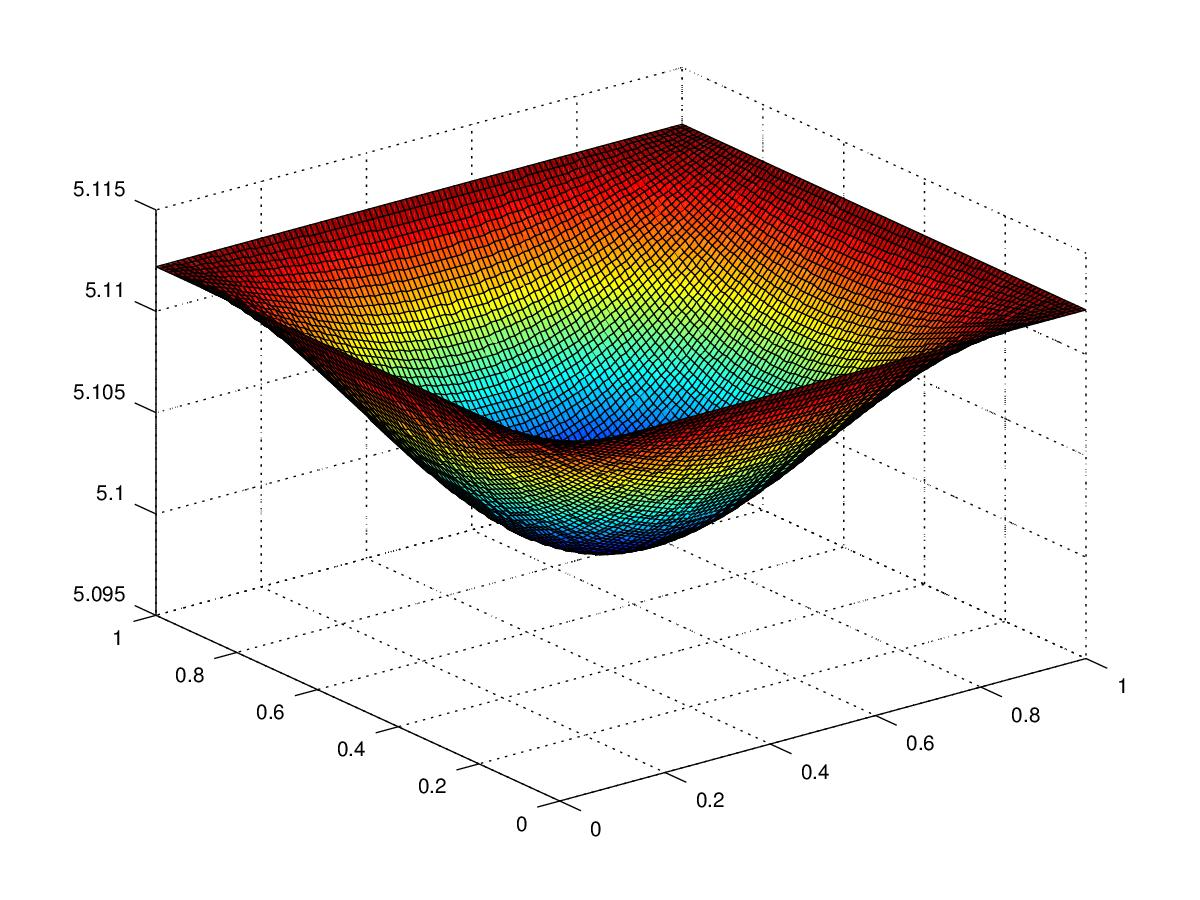
\includegraphics[width=0.8\textwidth]{v1_100-100.jpg}
    \caption{Gráfico solução da Validação 1 para $n = 100$ e $m = 100$}
    \label{fig:v1_100-100}
\end{figure}

\subsection{Validação 2 - Problema com solução conhecida}
Neste experimento, deve-se determinar a solução aproximada para $u(x,y)$ em 
$\Omega = (0,1) \times (0,1)$ considerando na Eq.
\eqref{eq:transporte}:
\begin{align}\label{eq:v2}
k &= 1\nonumber \\
\beta_x(x,y) &= 1\nonumber \\
\beta_y(x,y) &= 20y\nonumber \\
\gamma(x,y) &= 1\nonumber \\
f(x,y) \text{ tal que } u(x,y) &= 10xy(1-x)(1-y)e^{x^{4.5}}\\
&\text{ é a solução exata }\nonumber
\end{align}

e sabendo que $u(x,y) = 0$ no contorno de $\Omega$.

Veja na tabela \ref{tab:tv2} os tempos de execução deste experimento por 
valores $n$ e $m$ e versão do algoritmo SOR.

\begin{table}[ht]
\centering
\begin{tabular}{|c|c|l|c|}
\hline 
\textbf{n} & \textbf{m} & \textbf{SOR} & \textbf{Tempo} \\
\hline
\multirow{2}{*}{25}    & \multirow{2}{*}{100}   & normal & 0m0.041s \\
                       &                        & livre  & 0m1.695s \\
\hline
\multirow{2}{*}{100}   & \multirow{2}{*}{100}   & normal & 0m0.162s \\
                       &                        & livre  & 0m9.440s \\
\hline
\multirow{2}{*}{500}   & \multirow{2}{*}{1000}  & normal & 3m34.692s \\
                       &                        & livre  & $\infty$ \\
\hline
\multirow{2}{*}{1000}  & \multirow{2}{*}{10000} & normal & $\infty$ \\
                       &                        & livre  & $\infty$ \\
\hline
\end{tabular}
\caption{Testes - Validação 2}
\label{tab:tv2}
\end{table}

Veja na figura \ref{fig:v2_25-25} o gráfico da solução encontrada ao aplicar 
a Validação 2 para $\Omega = (0,1)\times(0,1)$, $n = 25$ e $m = 25$, e na 
figura \ref{fig:v2_80-100} o gráfico da solução encontrada ao aplicar 
a Validação 2 para $\Omega = (0,1)\times(0,1)$, $n = 80$ e $m = 100$.

\begin{figure}[h]
    \centering
    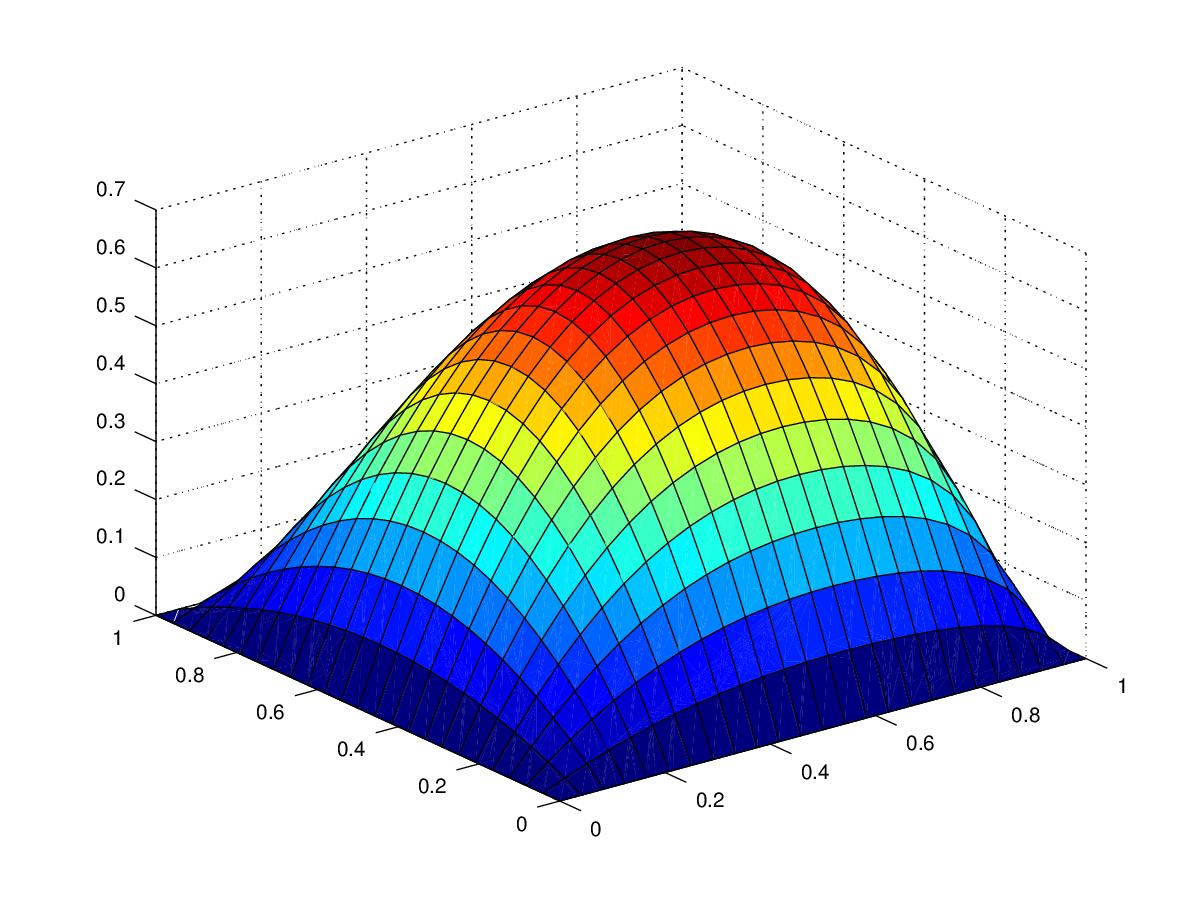
\includegraphics[width=0.8\textwidth]{v2_25-25}
    \caption{Gráfico solução da Validação 2 para $n = 25$ e $m = 25$}
    \label{fig:v2_25-25}
\end{figure}

\begin{figure}[h]
    \centering
    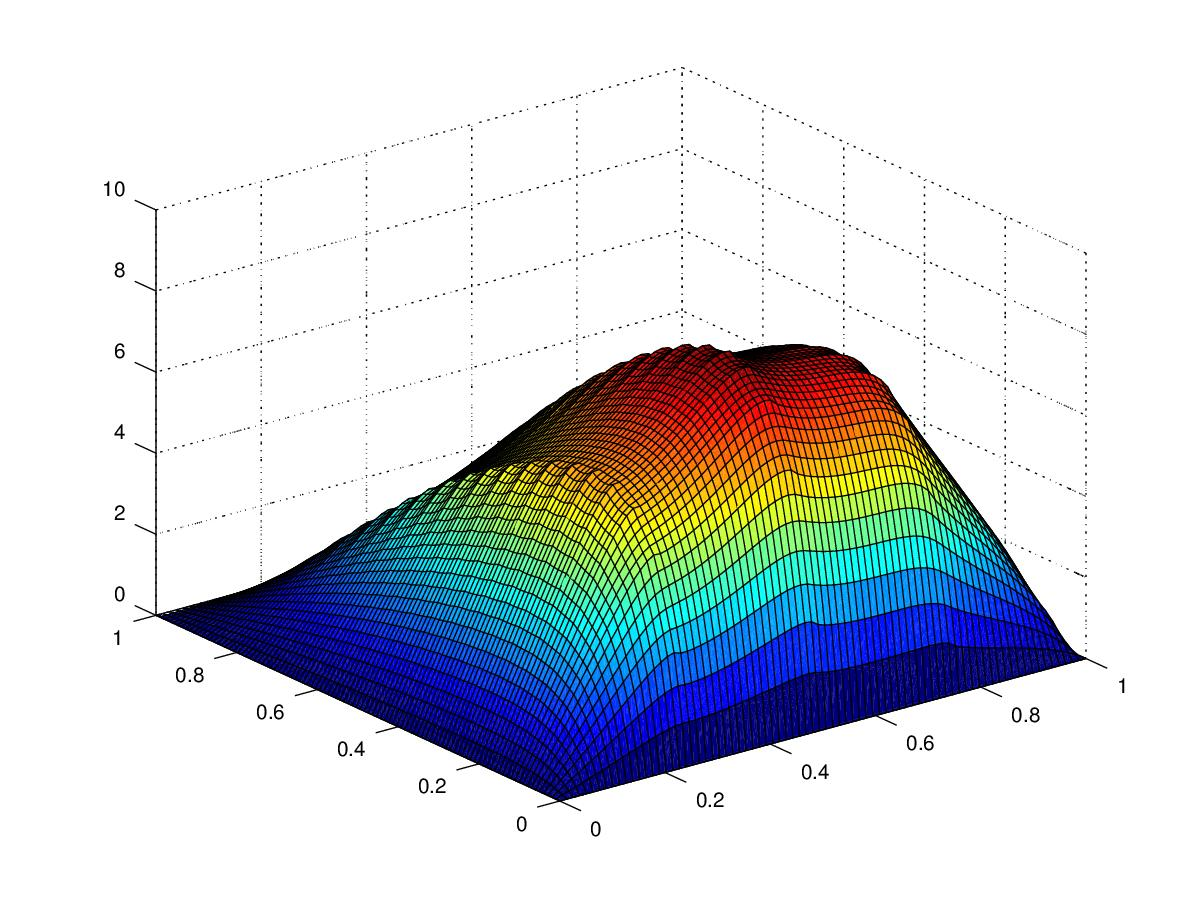
\includegraphics[width=0.8\textwidth]{v2_80-100}
    \caption{Gráfico solução da Validação 2 para $n = 80$ e $m = 100$}
    \label{fig:v2_80-100}
\end{figure}

\subsection{Aplicação Física 1 - Resfriador bidimensional} \label{sec:a1}
Este experimento consiste em uma aplicação dos métodos em questão para resfriar 
uma massa aquecida. Exemplos podem incluir o resfriamento de chips de 
computadores ou amplificadores elétricos. O modelo matemático que descreve a 
transferência de calor nas direções $x$ e $y$ é dado por:
\begin{equation} \label{eq:a1}
- k\left(\frac{\partial^2 u}{\partial x^2} + \frac{\partial^2 u}{\partial 
y^2}\right) + \frac{2c}{T}u = \frac{2c}{T}u_{ref} = 0 \text{   em   }
\Omega = (0,L) \times (0, W)
\end{equation}

\noindent onde $k$ é a condutividade térmica constante, $c$ é o coeficiente 
de transferência de calor, $T$ é a altura do resfriador e $u_{ref}$ é a 
temperatura de referência. Deve-se encontrar a temperatura no interior do 
resfriador considerando as seguintes condições de contorno:
\begin{align*}
u(x,0) &= 70\\
u(x,W) &= 70\\
u(0,y) &= 200\\
k\frac{\partial u}{\partial n}(L,y) &= c(u_{ref} - u(L,y))
\end{align*}

Veja na tabela \ref{tab:taf1} os tempos de execução deste experimento por 
valores $n$ e $m$ e versão do algoritmo SOR.

\begin{table}[ht]
\centering
\begin{tabular}{|c|c|l|c|}
\hline 
\textbf{n} & \textbf{m} & \textbf{SOR} & \textbf{Tempo} \\
\hline
\multirow{2}{*}{25}    & \multirow{2}{*}{100}   & normal & 0m0.041s \\
                       &                        & livre  & 0m0.095s \\
\hline
\multirow{2}{*}{100}   & \multirow{2}{*}{100}   & normal & 0m0.240s \\
                       &                        & livre  & 0m0.580s \\
\hline
\multirow{2}{*}{500}   & \multirow{2}{*}{1000}  & normal & 2m52.629s \\
                       &                        & livre  & 6m55.552s \\
\hline
\multirow{2}{*}{1000}  & \multirow{2}{*}{10000} & normal & 56m43.129s \\
                       &                        & livre  & 145m59.439s \\
\hline
\end{tabular}
\caption{Testes - Aplicação Física 1}
\label{tab:taf1}
\end{table}

Veja na figura \ref{fig:a1_25-25} o gráfico da solução encontrada ao aplicar 
a Aplicação Física 1 para $\Omega = (0,1)\times(0,1)$, $n = 25$ e $m = 25$, e 
na figura \ref{fig:a1_25-100} o gráfico da solução encontrada ao aplicar 
a Aplicação Física 1 para $\Omega = (0,1)\times(0,1)$, $n = 25$ e $m = 100$.

\begin{figure}[h]
    \centering
    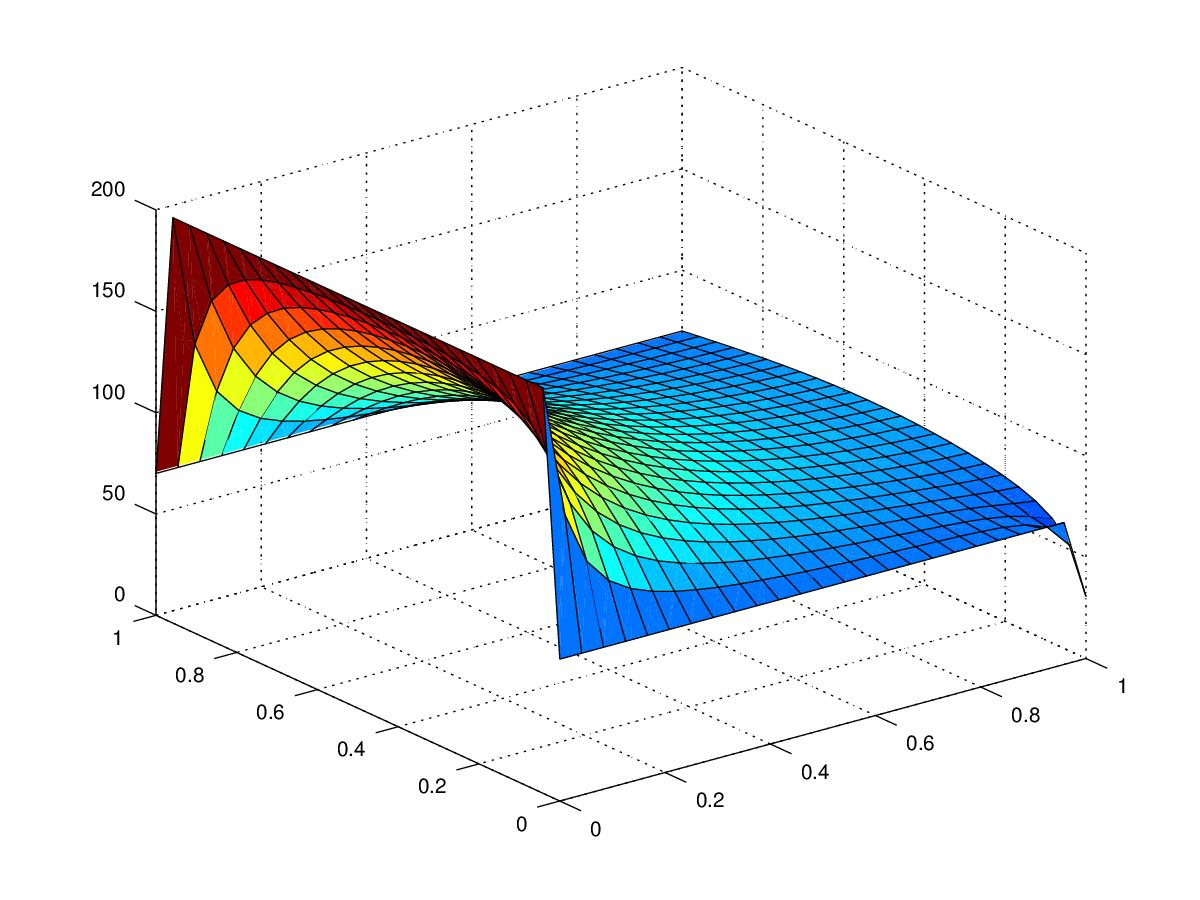
\includegraphics[width=0.8\textwidth]{a1_25-25}
    \caption{Gráfico solução da Aplicação Física 1 para $n = 25$ e $m = 25$}
    \label{fig:a1_25-25}
\end{figure}

\begin{figure}[h]
    \centering
    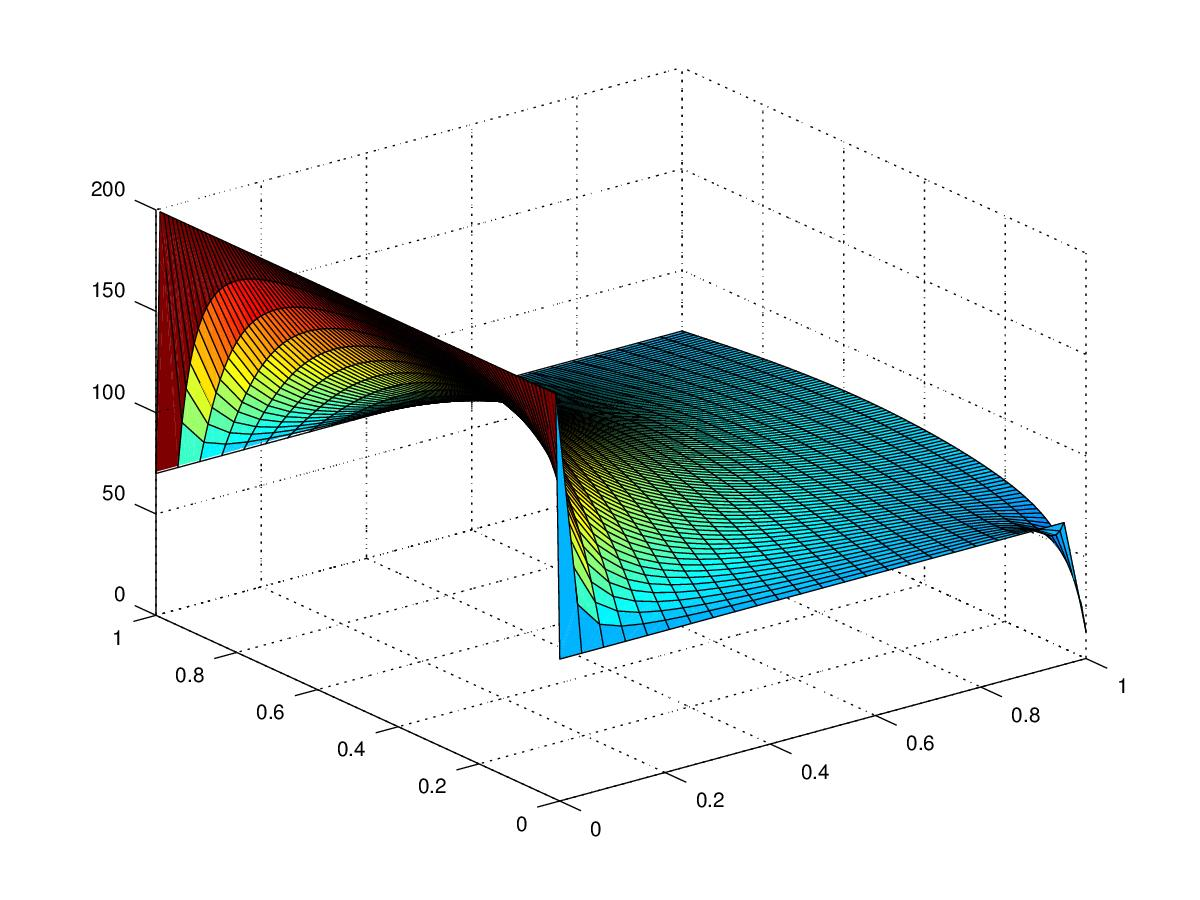
\includegraphics[width=0.8\textwidth]{a1_25-100}
    \caption{Gráfico solução da Aplicação Física 1 para $n = 25$ e $m = 100$}
    \label{fig:a1_25-100}
\end{figure}

Em ambos os testes anteriores, foi-se aplicado a condição de contorno mista. 
Caso seja aplicado a condição de contorno de valor prescrito $u(L, y) =
70$, e utilizando os dados $\Omega = (0,1)\times(0,1)$, $n = 25$ e $m = 100$, 
teremos um gráfico de solução ilustrado pela figura \ref{fig:a170_25-100}

\begin{figure}[h]
    \centering
    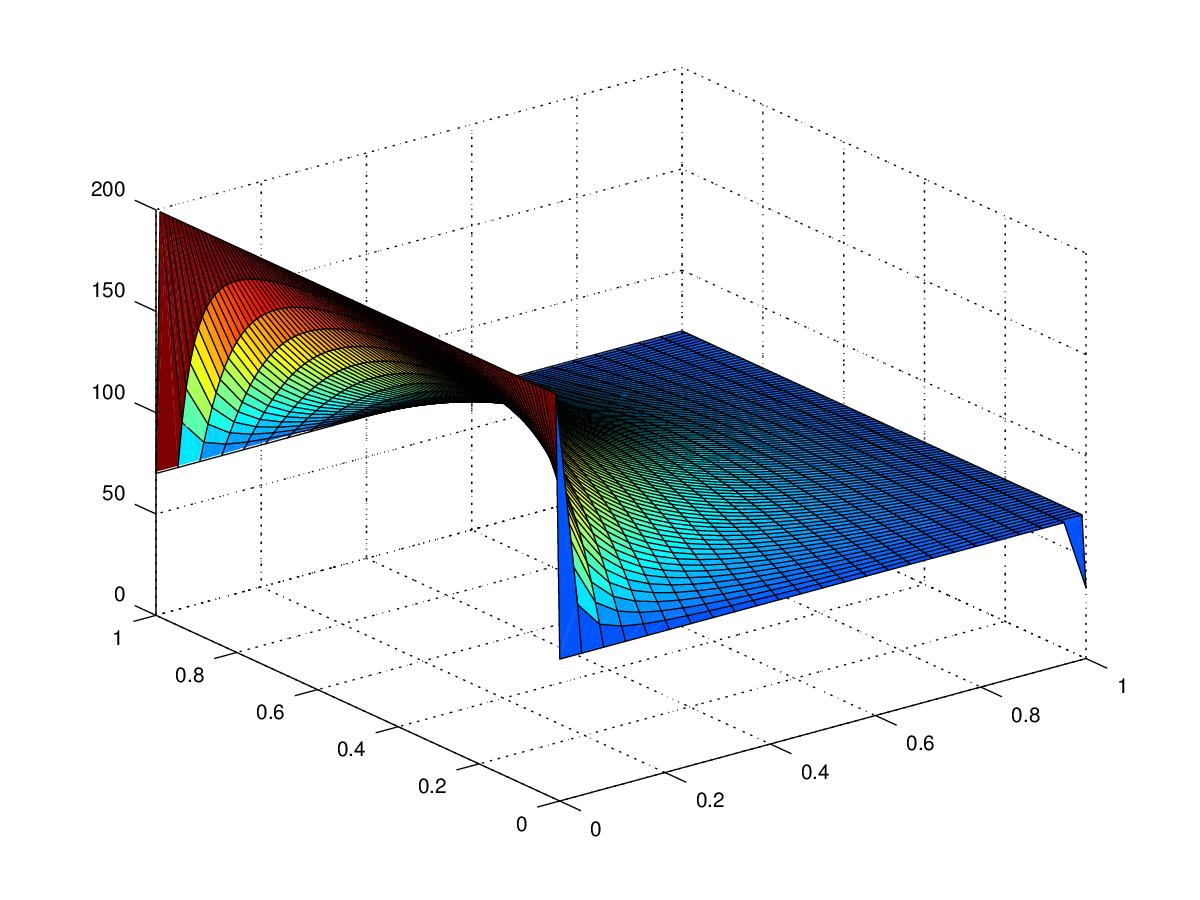
\includegraphics[width=0.8\textwidth]{a170_25-100}
    \caption{Gráfico solução da Aplicação Física 1 para $n = 25$ e $m = 100$ e 
$u(L, y) = 70$}
    \label{fig:a170_25-100}
\end{figure}

Podemos ver que as soluções encontradas para $n = 25$ e $m = 100$ modificando a 
condição de contorno são muito similares. Inclusive, a norma da solução é igual 
à 200.00 em ambos os casos. Um fato importante é notar que o caso de valor 
prescrito convergiu mais rapidamente (808 contra 1040 iterações do SOR).

\subsection{Aplicação Física 2 - Escoamento em Águas Subterrâneas}
Infelizmente não foi possível realizar este experimento.

% ------------------------------------------------------------------------------
% Conclusão
% ------------------------------------------------------------------------------
\section{Conclusão}
Com os dados coletados dos experimentos realizados, é passível assertar que a 
forma de armazenamento das estruturas resultantes pela discretização da equação 
\eqref{eq:transporte} por diferenças finitas tem um impacto muito significativo 
no tempo de processamento.

Notamos que ao utilizar uma estrutura específica de armazenamento da matriz 
penta-diagonal com os coeficientes computados de acordo, e igualmente para o 
vetor independente, temos um ganho em eficiência significativo se avaliado em 
relação a um programa livre de matriz. Isto é intuitivo, uma vez que o 
algoritmo SOR livre de matriz deverá realizar exaustivamente operações iguais 
em cada iteração, enquanto no outro caso tais cálculos são efetuados apenas 
uma vez e armazenados em uma estrutura apropriada. E desta estrutura, o acesso 
é direto, o que é um ganho considerável à realizar operações a cada passo.

Porém vale destacar que o algoritmo ``perdedor'' em tempo de processamento, o 
SOR livre de matriz, não é descartável. Este é uma opção para casos onde a 
quantidade de dados a serem processados é de proporções muito grandes. Nestes 
casos, o método rápido não pode ser aplicado pois necessita de espaço em 
memória para armazenar seus dados, restando assim a aplicação de um algoritmo 
livre de matriz eficiente para a solução do problema.

\end{document}
